% Preamble
\documentclass[11pt]{article}

% Packages
\usepackage{amsmath}
\usepackage{amssymb}
\usepackage{tikz}
\usetikzlibrary{arrows,arrows.meta,positioning,calc,petri}
\usepackage{adjustbox}
\usepackage{enumitem}
\usepackage{listings}
\usepackage[ruled,vlined]{algorithm2e}
\SetKwRepeat{Do}{do}{until}%
\newtheorem{theorem}{Theorem}

% Document
\begin{document}

    \section*{Rule R: Atomic post-agglomerable producer}
    Rule~R is similar to a post agglomeration rule and a formal description of Rule~R is in Figure~\ref{fig:rule_r}.
    In Rule~R we look for a place $p_0$ with a producer $t_0$ such that $t_0$ can always be followed by
    a firing of any consumer of $p_0$ without inhibiting other transitions or affecting places in $places(\varphi)$.
    The producer $t_0$ is then replaced with new transitions, one for each consumer, and these new transitions
    combine the effect of firing $t_0$ and the given consumer.
    Similarly to an agglomeration rule, Rule~R removes interleavings despite potentially increasing the size of the Petri net.
    However, Rule~R is more general, since it only operates on one producer at a time and leaves $p_0$ untouched,
    allowing tokens in $p_0$ in the initial marking, which a post agglomeration does not.
    Additionally, Rule~R does not require the weights of the arcs to and from the agglomerated place to be equal,
    making R usable in many cases.

    \begin{figure}[h!]
        \begin{adjustbox}{center}
            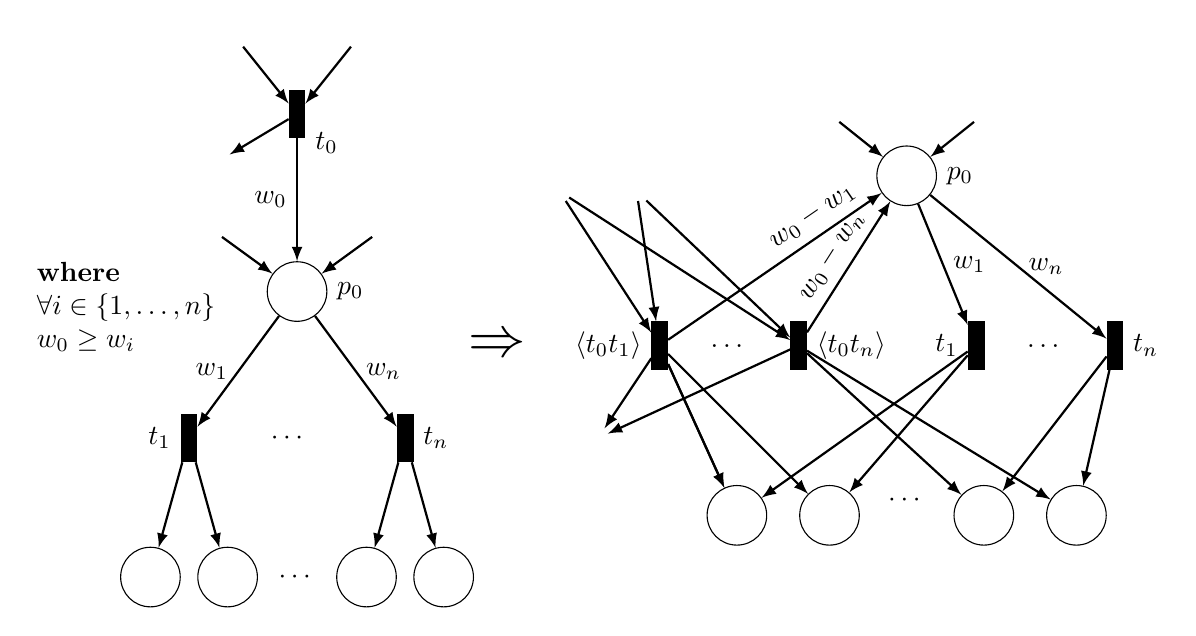
\begin{tikzpicture}[scale=0.98]
                % Left places
                \node[place,label=right:$p_0$] (rp) at (0.1,.7) {};
                \node[] (rph1) at (-.7,4) {};
                \node[] (rph2) at (.9,4) {};
                \node[] (rph1out) at (-.9,2.4) {};
                \node[place] (rpf1) at (-1.8,-3) {};
                \node[place] (rpf2) at (-0.8,-3) {};
                \node[place] (rpf3) at (1,-3) {};
                \node[place] (rpf4) at (2,-3) {};
                \node at (0.1,-3) {$\cdots$};

                % Left transitions
                \node[transition,minimum height=6mm,minimum width=2mm,fill=black,label=below right:$t_0$] (rh) at (0.1,3) {};
                \node[] (rh2) at (-1,1.5) {};
                \node[] (rh3) at (1.2,1.5) {};
                \node[transition,minimum height=6mm,minimum width=2mm,fill=black,label=left:$t_1$] (rf1) at (-1.3,-1.2) {};
                \node[transition,minimum height=6mm,minimum width=2mm,fill=black,label=right:$t_n$] (rf2) at (1.5,-1.2) {};
                \node at (0,-1.2) {$\cdots$};

                % Left arcs
                \draw[-latex,thick] (rph1) -- (rh);
                \draw[-latex,thick] (rph2) -- (rh);
                \draw[-latex,thick] (rh) edge node[left] {$w_0$} (rp);
                \draw[-latex,thick] (rh) -- (rph1out);
                \draw[-latex,thick] (rh2) -- (rp);
                \draw[-latex,thick] (rh3) -- (rp);
                \draw[-latex,thick] (rp) edge node[left] {$w_1$} (rf1);
                \draw[-latex,thick] (rp) edge node[right] {$w_n$} (rf2);
                \draw[-latex,thick] (rf1) -- (rpf1);
                \draw[-latex,thick] (rf1) -- (rpf2);
                \draw[-latex,thick] (rf2) -- (rpf3);
                \draw[-latex,thick] (rf2) -- (rpf4);

                % ================== Middle arrow ==================
                \node (arrow) at (2.7,0) {\huge$\Rightarrow$};
                % ==================================================

                % Right places
                \node[] (lph1) at (3.5,2) {};
                \node[] (lph2) at (4.5,2) {};
                \node[] (lhout) at (4,-1.2) {};
                \node[place,label=right:$p_0$] (lp) at (8,2.2) {};
                \node[place] (lpf1) at (5.8,-2.2) {};
                \node[place] (lpf2) at (7,-2.2) {};
                \node[place] (lpf3) at (9,-2.2) {};
                \node[place] (lpf4) at (10.2,-2.2) {};
                \node at (8,-2) {$\cdots$};

                % Right transitions
                \node (lh2) at (7,3) {};
                \node (lh3) at (9,3) {};
                \node[transition,minimum height=6mm,minimum width=2mm,fill=black,label=left:$\langle t_0t_1\rangle$] (lhf1f1) at (4.8,0) {};
                \node at (5.7,0) {$\dots$};
                \node[transition,minimum height=6mm,minimum width=2mm,fill=black,label=right:$\langle t_0t_n\rangle$] (lhf2f2) at (6.6,0) {};
                \node[transition,minimum height=6mm,minimum width=2mm,fill=black,label=left:$t_1$] (lf1) at (8.9,0) {};
                \node at (9.8,0) {$\dots$};
                \node[transition,minimum height=6mm,minimum width=2mm,fill=black,label=right:$t_n$] (lf2) at (10.7,0) {};

                % Right arcs above
                \draw[-latex,thick] (lhf1f1) edge[sloped, above right] node {$w_0-w_1$} (lp);
                \draw[-latex,thick] (lhf2f2) edge[sloped, above] node {$w_0-w_n$} (lp);
                \draw[-latex,thick] (lph1) -- (lhf1f1);
                \draw[-latex,thick] (lph1) -- (lhf2f2);
                \draw[-latex,thick] (lph2) -- (lhf1f1);
                \draw[-latex,thick] (lph2) -- (lhf2f2);
                \draw[-latex,thick] (lh2) -- (lp);
                \draw[-latex,thick] (lh3) -- (lp);
                \draw[-latex,thick] (lp) edge node[right] {$w_1$} (lf1);
                \draw[-latex,thick] (lp) edge node[right] {$w_n$} (lf2);

                % Right arcs below
                \draw[-latex,thick] (lhf1f1) -- (lhout);
                \draw[-latex,thick] (lhf2f2) -- (lhout);
                \draw[-latex,thick] (lhf1f1) -- (lpf1);
                \draw[-latex,thick] (lhf1f1) -- (lpf1);
                \draw[-latex,thick] (lhf1f1) -- (lpf2);
                \draw[-latex,thick] (lhf2f2) -- (lpf3);
                \draw[-latex,thick] (lhf2f2) -- (lpf4);
                \draw[-latex,thick] (lf1) -- (lpf1);
                \draw[-latex,thick] (lf1) -- (lpf2);
                \draw[-latex,thick] (lf2) -- (lpf3);
                \draw[-latex,thick] (lf2) -- (lpf4);

                % Right labels with background
                %\node[above=3pt of lhf1f1,outer sep=1pt,fill=white] {$h f_1\dots f_1$};
                %\node[above=3pt of lhf2f2,outer sep=1pt,fill=white] {$h f_2\dots f_2$};

                % Right lower weights
                \node[text width=7cm] at (.3,0.5) {\textbf{where }\\ $\forall i\in\{1,\dotsc,n\}$\\$w_0\geq w_i$};

            \end{tikzpicture}
        \end{adjustbox}
        \vspace{5mm}

        \begin{adjustbox}{center}
            \begin{tabular}{|p{68mm}|p{75mm}|} \hline
            Precondition & Update \\ \hline
            Fix place $p_0$ and transition $t_0$ s.t.:
            \begin{itemize}[leftmargin=10mm]
                \item[R1)] $t_0\in {}^\bullet p_0\land p_0^\bullet\neq\emptyset$
                \item[R2)] $^\bullet p_0 \cap p_0^\bullet = \emptyset$
                \item[R3)] $p_0 ^\circ = {}^\circ (p_0^\bullet) = ((p_0^\bullet)^\bullet)^\circ = \emptyset$
                \item[R4)] $(\{p_0\} \cup (p_0^\bullet)^\bullet) \cap places(\varphi) = \emptyset$
                \item[R5)] ${}^\bullet (p_0^\bullet)=\{p_0\}$
                \item[R6)] $\boxplus(t_0, p_0)\geq \boxminus(p_0,t)$ for all $t\in p_0^\bullet$
            \end{itemize} &

            \begin{itemize}[leftmargin=10mm]
                \item[UR1)]
                For each transition $t \in p_0^\bullet$ create a transition $\langle t_0 t\rangle$ with the following arcs:

                $\boxminus(\langle t_0 t\rangle)=\boxminus(t_0)$

                $\boxplus(\langle t_0 t\rangle)=\boxplus(t_0)+\boxplus(t)-\boxminus(t)$

                $I(\langle t_0 t\rangle)=I(t_0)$

                \item[UR2)] Remove $t_0$
            \end{itemize} \\ \hline
            \end{tabular}
        \end{adjustbox}
        \caption{Rule R: Atomic post-agglomerable producer}
        \label{fig:rule_r}
    \end{figure}

    \begin{theorem}
        Rule~R in Figure~\ref{fig:rule_r} is correct for LTL\textbackslash X.
    \end{theorem}

\end{document}
